\begin{figure}[H]
    \centering
    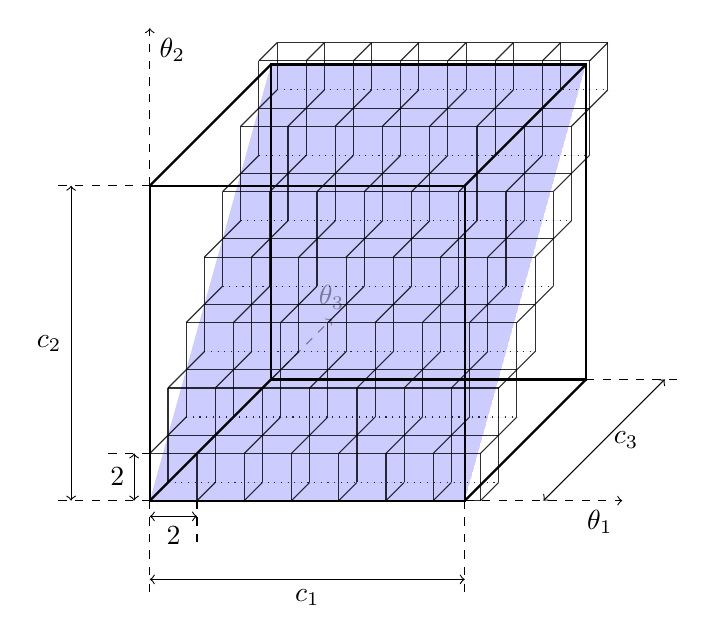
\begin{tikzpicture}[scale=2]
        % Define the cube's vertices
        \coordinate (A) at (0,0,0);
        \coordinate (B) at (2,0,0);
        \coordinate (C) at (2,2,0);
        \coordinate (D) at (0,2,0);
        \coordinate (E) at (0,0,2);
        \coordinate (F) at (2,0,2);
        \coordinate (G) at (2,2,2);
        \coordinate (H) at (0,2,2);

        % Draw the shaded area under the hypercube
        \begin{scope}
            \clip (D) -- (E) -- (F) -- (C);
            \fill[blue!20] (D) -- (E) -- (F) -- (C);
        \end{scope}
        
        % Draw the front face
        \draw[thick] (A) -- (B) -- (C) -- (D) -- cycle;

        % Draw the back face
        \draw[thick] (E) -- (F) -- (G) -- (H) -- cycle;

        % Draw the connecting edges
        \draw[thick] (A) -- (E);
        \draw[thick] (B) -- (F);
        \draw[thick] (C) -- (G);
        \draw[thick] (D) -- (H);
    
        % Label the axes
        \draw[->, dashed] (0,0,2) -- (3,0,2) node[anchor=north east] {$\theta_1$};
        \draw[->, dashed] (0,0,2) -- (0,3,2) node[anchor=north west] {$\theta_2$};
        \draw[->, dashed,opacity=0.4] (0,0,0) -- (0,0,-1) node[anchor=south] {$\theta_3$};
        
        \draw[<->] (0,-0.1,2)  -- (0.3,-0.1,2) node[midway, below]{$2\vep$};
        \draw[<->] (-0.1,0,2)  -- (-0.1,0.3,2) node[midway, left]{$2\vep$};
        \draw[dashed] (0,0.3,2)  -- (-0.3,0.3,2);
        \draw[dashed] (0.3,0,2)  -- (0.3,-0.3,2);
        
        \draw[<->] (0,-0.5,2)  -- (2,-0.5,2) node[midway, below]{$c_1$};
        \draw[<->] (-0.5,0,2)  -- (-0.5,2,2) node[midway, left]{$c_2$};
        \draw[<->] (2.5,0,2)   -- (2.5,0,0)  node[midway, right]{$c_3$};
        \draw[dashed] (0,0,2)  -- (-0.6,0,2);
        \draw[dashed] (0,2,2)  -- (-0.6,2,2);
        \draw[dashed] (0,0,2)  -- (0,-0.6,2);
        \draw[dashed] (2,0,2)  -- (2,-0.6,2);
        \draw[dashed] (2,0,0)  -- (2.6,0,0);
        
        % Draw the p-norm balls which cover the hypercube
        \draw[opacity=0.8, fill=blue!50] (0.3,0,2)   -- (0.3,0.3,2);
        \draw[opacity=0.8, fill=blue!50] (0.3,0,2)   -- (0.3,0,1.7);
        \draw[opacity=0.8, fill=blue!50] (0.6,0,2)   -- (0.6,0.3,2);
        \draw[opacity=0.8, fill=blue!50] (0.6,0,2)   -- (0.6,0,1.7);
        \draw[opacity=0.8, fill=blue!50] (0.9,0,2)   -- (0.9,0.3,2);
        \draw[opacity=0.8, fill=blue!50] (0.9,0,2)   -- (0.9,0,1.7);
        \draw[opacity=0.8, fill=blue!50] (1.2,0,2)   -- (1.2,0.3,2);
        \draw[opacity=0.8, fill=blue!50] (1.2,0,2)   -- (1.2,0,1.7);
        \draw[opacity=0.8, fill=blue!50] (1.5,0,2)   -- (1.5,0.3,2);
        \draw[opacity=0.8, fill=blue!50] (1.5,0,2)   -- (1.5,0,1.7);
        \draw[opacity=0.8, fill=blue!50] (1.8,0,2)   -- (1.8,0.3,2);
        \draw[opacity=0.8, fill=blue!50] (1.8,0,2)   -- (1.8,0,1.7);
        \draw[opacity=0.8, fill=blue!50] (2.1,0,2)   -- (2.1,0.3,2);
        \draw[opacity=0.8, fill=blue!50] (2.1,0,2)   -- (2.1,0,1.7);
        
        \draw[opacity=0.8, fill=blue!50] (0,0.3,2)   -- (0,0.3,1.4);
        \draw[opacity=0.8, fill=blue!50] (0.3,0.3,2) -- (0.3,0.3,1.4);
        \draw[opacity=0.8, fill=blue!50] (0.6,0.3,2) -- (0.6,0.3,1.4);
        \draw[opacity=0.8, fill=blue!50] (0.9,0.3,2) -- (0.9,0.3,1.4);
        \draw[opacity=0.8, fill=blue!50] (1.2,0.3,2) -- (1.2,0.3,1.4);
        \draw[opacity=0.8, fill=blue!50] (1.5,0.3,2) -- (1.5,0.3,1.4);
        \draw[opacity=0.8, fill=blue!50] (1.8,0.3,2) -- (1.8,0.3,1.4);
        \draw[opacity=0.8, fill=blue!50] (2.1,0.3,2) -- (2.1,0.3,1.4);
        \draw[opacity=0.8, fill=blue!50] (0,0,1.7)   -- (0,0.6,1.7);
        \draw[opacity=0.8, fill=blue!50] (0.3,0,1.7) -- (0.3,0.6,1.7);
        \draw[opacity=0.8, fill=blue!50] (0.6,0,1.7) -- (0.6,0.6,1.7);
        \draw[opacity=0.8, fill=blue!50] (0.9,0,1.7) -- (0.9,0.6,1.7);
        \draw[opacity=0.8, fill=blue!50] (1.2,0,1.7) -- (1.2,0.6,1.7);
        \draw[opacity=0.8, fill=blue!50] (1.5,0,1.7) -- (1.5,0.6,1.7);
        \draw[opacity=0.8, fill=blue!50] (1.8,0,1.7) -- (1.8,0.6,1.7);
        \draw[opacity=0.8, fill=blue!50] (2.1,0,1.7) -- (2.1,0.6,1.7);
        \draw[opacity=0.8, fill=blue!50] (0,0.6,1.7) -- (0,0.6,1.1);
        \draw[opacity=0.8, fill=blue!50] (0.3,0.6,1.7) -- (0.3,0.6,1.1);
        \draw[opacity=0.8, fill=blue!50] (0.6,0.6,1.7) -- (0.6,0.6,1.1);
        \draw[opacity=0.8, fill=blue!50] (0.9,0.6,1.7) -- (0.9,0.6,1.1);
        \draw[opacity=0.8, fill=blue!50] (1.2,0.6,1.7) -- (1.2,0.6,1.1);
        \draw[opacity=0.8, fill=blue!50] (1.5,0.6,1.7) -- (1.5,0.6,1.1);
        \draw[opacity=0.8, fill=blue!50] (1.8,0.6,1.7) -- (1.8,0.6,1.1);
        \draw[opacity=0.8, fill=blue!50] (2.1,0.6,1.7) -- (2.1,0.6,1.1);
        \draw[opacity=0.8, fill=blue!50] (0,0.3,1.4) -- (0,0.9,1.4);
        \draw[opacity=0.8, fill=blue!50] (0.3,0.3,1.4) -- (0.3,0.9,1.4);
        \draw[opacity=0.8, fill=blue!50] (0.6,0.3,1.4) -- (0.6,0.9,1.4);
        \draw[opacity=0.8, fill=blue!50] (0.9,0.3,1.4) -- (0.9,0.9,1.4);
        \draw[opacity=0.8, fill=blue!50] (1.2,0.3,1.4) -- (1.2,0.9,1.4);
        \draw[opacity=0.8, fill=blue!50] (1.5,0.3,1.4) -- (1.5,0.9,1.4);
        \draw[opacity=0.8, fill=blue!50] (1.8,0.3,1.4) -- (1.8,0.9,1.4);
        \draw[opacity=0.8, fill=blue!50] (2.1,0.3,1.4) -- (2.1,0.9,1.4);
        \draw[opacity=0.8, fill=blue!50] (0,0.9,1.4) -- (0,0.9,0.8);
        \draw[opacity=0.8, fill=blue!50] (0.3,0.9,1.4) -- (0.3,0.9,0.8);
        \draw[opacity=0.8, fill=blue!50] (0.6,0.9,1.4) -- (0.6,0.9,0.8);
        \draw[opacity=0.8, fill=blue!50] (0.9,0.9,1.4) -- (0.9,0.9,0.8);
        \draw[opacity=0.8, fill=blue!50] (1.2,0.9,1.4) -- (1.2,0.9,0.8);
        \draw[opacity=0.8, fill=blue!50] (1.5,0.9,1.4) -- (1.5,0.9,0.8);
        \draw[opacity=0.8, fill=blue!50] (1.8,0.9,1.4) -- (1.8,0.9,0.8);
        \draw[opacity=0.8, fill=blue!50] (2.1,0.9,1.4) -- (2.1,0.9,0.8);
        \draw[opacity=0.8, fill=blue!50] (0,0.6,1.1) -- (0,1.2,1.1);
        \draw[opacity=0.8, fill=blue!50] (0.3,0.6,1.1) -- (0.3,1.2,1.1);
        \draw[opacity=0.8, fill=blue!50] (0.6,0.6,1.1) -- (0.6,1.2,1.1);
        \draw[opacity=0.8, fill=blue!50] (0.9,0.6,1.1) -- (0.9,1.2,1.1);
        \draw[opacity=0.8, fill=blue!50] (1.2,0.6,1.1) -- (1.2,1.2,1.1);
        \draw[opacity=0.8, fill=blue!50] (1.5,0.6,1.1) -- (1.5,1.2,1.1);
        \draw[opacity=0.8, fill=blue!50] (1.8,0.6,1.1) -- (1.8,1.2,1.1);
        \draw[opacity=0.8, fill=blue!50] (2.1,0.6,1.1) -- (2.1,1.2,1.1);
        \draw[opacity=0.8, fill=blue!50] (0,1.2,1.1) -- (0,1.2,0.5);
        \draw[opacity=0.8, fill=blue!50] (0.3,1.2,1.1) -- (0.3,1.2,0.5);
        \draw[opacity=0.8, fill=blue!50] (0.6,1.2,1.1) -- (0.6,1.2,0.5);
        \draw[opacity=0.8, fill=blue!50] (0.9,1.2,1.1) -- (0.9,1.2,0.5);
        \draw[opacity=0.8, fill=blue!50] (1.2,1.2,1.1) -- (1.2,1.2,0.5);
        \draw[opacity=0.8, fill=blue!50] (1.5,1.2,1.1) -- (1.5,1.2,0.5);
        \draw[opacity=0.8, fill=blue!50] (1.8,1.2,1.1) -- (1.8,1.2,0.5);
        \draw[opacity=0.8, fill=blue!50] (2.1,1.2,1.1) -- (2.1,1.2,0.5);
        \draw[opacity=0.8, fill=blue!50] (0,0.9,0.8) -- (0,1.5,0.8);
        \draw[opacity=0.8, fill=blue!50] (0.3,0.9,0.8) -- (0.3,1.5,0.8);
        \draw[opacity=0.8, fill=blue!50] (0.6,0.9,0.8) -- (0.6,1.5,0.8);
        \draw[opacity=0.8, fill=blue!50] (0.9,0.9,0.8) -- (0.9,1.5,0.8);
        \draw[opacity=0.8, fill=blue!50] (1.2,0.9,0.8) -- (1.2,1.5,0.8);
        \draw[opacity=0.8, fill=blue!50] (1.5,0.9,0.8) -- (1.5,1.5,0.8);
        \draw[opacity=0.8, fill=blue!50] (1.8,0.9,0.8) -- (1.8,1.5,0.8);
        \draw[opacity=0.8, fill=blue!50] (2.1,0.9,0.8) -- (2.1,1.5,0.8);
        \draw[opacity=0.8, fill=blue!50] (0,1.5,0.8) -- (0,1.5,0.2);
        \draw[opacity=0.8, fill=blue!50] (0.3,1.5,0.8) -- (0.3,1.5,0.2);
        \draw[opacity=0.8, fill=blue!50] (0.6,1.5,0.8) -- (0.6,1.5,0.2);
        \draw[opacity=0.8, fill=blue!50] (0.9,1.5,0.8) -- (0.9,1.5,0.2);
        \draw[opacity=0.8, fill=blue!50] (1.2,1.5,0.8) -- (1.2,1.5,0.2);
        \draw[opacity=0.8, fill=blue!50] (1.5,1.5,0.8) -- (1.5,1.5,0.2);
        \draw[opacity=0.8, fill=blue!50] (1.8,1.5,0.8) -- (1.8,1.5,0.2);
        \draw[opacity=0.8, fill=blue!50] (2.1,1.5,0.8) -- (2.1,1.5,0.2);
        \draw[opacity=0.8, fill=blue!50] (0,1.2,0.5) -- (0,1.8,0.5);
        \draw[opacity=0.8, fill=blue!50] (0.3,1.2,0.5) -- (0.3,1.8,0.5);
        \draw[opacity=0.8, fill=blue!50] (0.6,1.2,0.5) -- (0.6,1.8,0.5);
        \draw[opacity=0.8, fill=blue!50] (0.9,1.2,0.5) -- (0.9,1.8,0.5);
        \draw[opacity=0.8, fill=blue!50] (1.2,1.2,0.5) -- (1.2,1.8,0.5);
        \draw[opacity=0.8, fill=blue!50] (1.5,1.2,0.5) -- (1.5,1.8,0.5);
        \draw[opacity=0.8, fill=blue!50] (1.8,1.2,0.5) -- (1.8,1.8,0.5);
        \draw[opacity=0.8, fill=blue!50] (2.1,1.2,0.5) -- (2.1,1.8,0.5);
        \draw[opacity=0.8, fill=blue!50] (0,1.8,0.5) -- (0,1.8,-0.1);
        \draw[opacity=0.8, fill=blue!50] (0.3,1.8,0.5) -- (0.3,1.8,-0.1);
        \draw[opacity=0.8, fill=blue!50] (0.6,1.8,0.5) -- (0.6,1.8,-0.1);
        \draw[opacity=0.8, fill=blue!50] (0.9,1.8,0.5) -- (0.9,1.8,-0.1);
        \draw[opacity=0.8, fill=blue!50] (1.2,1.8,0.5) -- (1.2,1.8,-0.1);
        \draw[opacity=0.8, fill=blue!50] (1.5,1.8,0.5) -- (1.5,1.8,-0.1);
        \draw[opacity=0.8, fill=blue!50] (1.8,1.8,0.5) -- (1.8,1.8,-0.1);
        \draw[opacity=0.8, fill=blue!50] (2.1,1.8,0.5) -- (2.1,1.8,-0.1);
        \draw[opacity=0.8, fill=blue!50] (0,1.5,0.2) -- (0,2.1,0.2);
        \draw[opacity=0.8, fill=blue!50] (0.3,1.5,0.2) -- (0.3,2.1,0.2);
        \draw[opacity=0.8, fill=blue!50] (0.6,1.5,0.2) -- (0.6,2.1,0.2);
        \draw[opacity=0.8, fill=blue!50] (0.9,1.5,0.2) -- (0.9,2.1,0.2);
        \draw[opacity=0.8, fill=blue!50] (1.2,1.5,0.2) -- (1.2,2.1,0.2);
        \draw[opacity=0.8, fill=blue!50] (1.5,1.5,0.2) -- (1.5,2.1,0.2);
        \draw[opacity=0.8, fill=blue!50] (1.8,1.5,0.2) -- (1.8,2.1,0.2);
        \draw[opacity=0.8, fill=blue!50] (2.1,1.5,0.2) -- (2.1,2.1,0.2);
        \draw[opacity=0.8, fill=blue!50] (0,2.1,0.2) -- (0,2.1,-0.1);
        \draw[opacity=0.8, fill=blue!50] (0.3,2.1,0.2) -- (0.3,2.1,-0.1);
        \draw[opacity=0.8, fill=blue!50] (0.6,2.1,0.2) -- (0.6,2.1,-0.1);
        \draw[opacity=0.8, fill=blue!50] (0.9,2.1,0.2) -- (0.9,2.1,-0.1);
        \draw[opacity=0.8, fill=blue!50] (1.2,2.1,0.2) -- (1.2,2.1,-0.1);
        \draw[opacity=0.8, fill=blue!50] (1.5,2.1,0.2) -- (1.5,2.1,-0.1);
        \draw[opacity=0.8, fill=blue!50] (1.8,2.1,0.2) -- (1.8,2.1,-0.1);
        \draw[opacity=0.8, fill=blue!50] (2.1,2.1,0.2) -- (2.1,2.1,-0.1);
        \draw[opacity=0.8, fill=blue!50] (0,1.8,-0.1) -- (0,2.1,-0.1);
        \draw[opacity=0.8, fill=blue!50] (0.3,1.8,-0.1) -- (0.3,2.1,-0.1);
        \draw[opacity=0.8, fill=blue!50] (0.6,1.8,-0.1) -- (0.6,2.1,-0.1);
        \draw[opacity=0.8, fill=blue!50] (0.9,1.8,-0.1) -- (0.9,2.1,-0.1);
        \draw[opacity=0.8, fill=blue!50] (1.2,1.8,-0.1) -- (1.2,2.1,-0.1);
        \draw[opacity=0.8, fill=blue!50] (1.5,1.8,-0.1) -- (1.5,2.1,-0.1);
        \draw[opacity=0.8, fill=blue!50] (1.8,1.8,-0.1) -- (1.8,2.1,-0.1);
        \draw[opacity=0.8, fill=blue!50] (2.1,1.8,-0.1) -- (2.1,2.1,-0.1);
        
        \draw[opacity=0.8, fill=blue!50] (0,0,2)     -- (2.1,0,2);
        
        \draw[opacity=0.8, fill=blue!50, dotted] (0,0,1.7)   -- (2.1,0,1.7);
        \draw[opacity=0.8, fill=blue!50] (0,0.3,2)   -- (2.1,0.3,2);
        \draw[opacity=0.8, fill=blue!50] (0,0.3,1.7) -- (2.1,0.3,1.7);
        \draw[opacity=0.8, fill=blue!50, dotted] (0,0.3,1.4)   -- (2.1,0.3,1.4);
        \draw[opacity=0.8, fill=blue!50] (0,0.6,1.7) -- (2.1,0.6,1.7);
        \draw[opacity=0.8, fill=blue!50] (0,0.6,1.4) -- (2.1,0.6,1.4);
        \draw[opacity=0.8, fill=blue!50, dotted] (0,0.6,1.1)   -- (2.1,0.6,1.1);
        \draw[opacity=0.8, fill=blue!50] (0,0.9,1.4) -- (2.1,0.9,1.4);
        \draw[opacity=0.8, fill=blue!50] (0,0.9,1.1) -- (2.1,0.9,1.1);
        \draw[opacity=0.8, fill=blue!50, dotted] (0,0.9,0.8)   -- (2.1,0.9,0.8);
        \draw[opacity=0.8, fill=blue!50] (0,1.2,1.1) -- (2.1,1.2,1.1);
        \draw[opacity=0.8, fill=blue!50] (0,1.2,0.8) -- (2.1,1.2,0.8);
        \draw[opacity=0.8, fill=blue!50, dotted] (0,1.2,0.5)   -- (2.1,1.2,0.5);
        \draw[opacity=0.8, fill=blue!50] (0,1.5,0.8) -- (2.1,1.5,0.8);
        \draw[opacity=0.8, fill=blue!50] (0,1.5,0.5) -- (2.1,1.5,0.5);
        \draw[opacity=0.8, fill=blue!50, dotted] (0,1.5,0.2)   -- (2.1,1.5,0.2);
        \draw[opacity=0.8, fill=blue!50] (0,1.8,0.5) -- (2.1,1.8,0.5);
        \draw[opacity=0.8, fill=blue!50] (0,1.8,0.2) -- (2.1,1.8,0.2);
        \draw[opacity=0.8, fill=blue!50, dotted] (0,1.8,-0.1)   -- (2.1,1.8,-0.1);
        \draw[opacity=0.8, fill=blue!50] (0,2.1,0.2) -- (2.1,2.1,0.2);
        \draw[opacity=0.8, fill=blue!50] (0,2.1,-0.1) -- (2.1,2.1,-0.1);
    \end{tikzpicture}
    \caption{The blue area represents $\Theta \defeq \set{(\theta_1, \theta_2, \theta_3)}[\theta_2 = \theta_3, \theta_i \in [a_i, a_i + c_i]] \subset \bbR^{3}$, and the small cubes represent the $\vep$-covering net of $\Theta$ w.r.t. $\norm{\cdot}_{\infty}$}
    \label{fig:covering-number-hypercube-correlations}
\end{figure}